\documentclass{article}
\usepackage{svg}
\usepackage{amsmath}
\usepackage{color} %red, green, blue, yellow, cyan, magenta, black, white
\definecolor{mygreen}{RGB}{28,172,0} % color values Red, Green, Blue
\definecolor{mylilas}{RGB}{170,55,241}
\usepackage{listings}
\usepackage[toc,page]{appendix}

\title{MATLAB Paris Law for Three Point Bending}
\author{Theron Guo}
\begin{document}
\maketitle
\chapter{Main}
The task was to find a good specimen geometry for our later experiments. For that I coded an easy MATLAB code where one defines some material parameters and can then calculate the critical crack length $a_{crit}$ and the number of cycles for the crack to grow from $a_{init}$ to $a_{crit}$ with Paris Law. 

\begin{figure}[htbp]
	\centering
	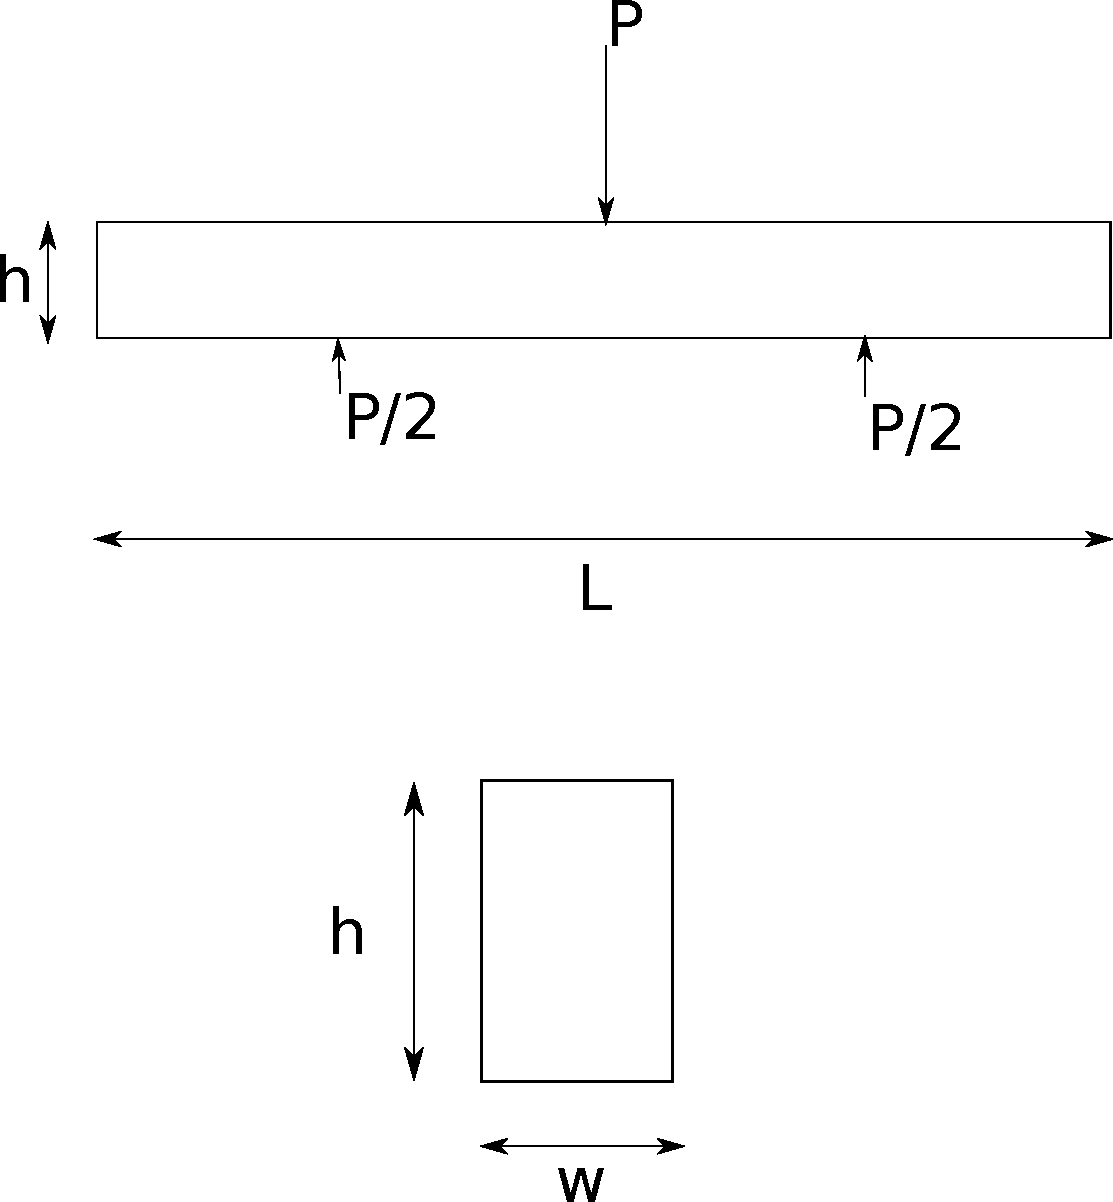
\includegraphics[width=0.5\textwidth]{output}
	\caption{Setup}
\end{figure}

The code is structured as follows: First, one has to decide which length, height and width of the specimen. Then one has to specify which material is used, i.e. $K_{Ic}$, the initial crack length $a_{init}$ and Paris law parameters $C$ and $m$.
Finally, the load $P$ has to be defined and the $\beta$ for the stress intensity factor $K$. Here, $\beta$ can be either constant or a function of the crack length $a$. If $\beta$ should be specified as a function, the user must pass three points of the curve into the \textit{calcBeta} function:
\begin{enumerate}
	\item $\beta$ at $a/h=0$
	\item $\beta$ at the minimum
	\item $\beta$ at $a/h=0.6$
\end{enumerate}

When the user has done that, he can start the script. First, $\sigma_{max}$ will be calculated from $$\sigma_{max}=\frac{M_{max}}{I}\cdot \frac{h}{2}=\frac{Pl/4}{bh^3/12}\cdot \frac{h}{2}=\frac{3}{2}P\frac{l}{bh^2}$$
With $\sigma_{max}$ the critical crack length is now calculated.
\begin{align}
K_{Ic}&=\beta\sigma_{max}\sqrt{\pi a_{crit}} \\
\Leftrightarrow a_{crit} &=\frac{1}{\pi}\frac{K^2_{Ic}}{\beta^2 \sigma^2_{max}}
\end{align}
With $a_{crit}$, we can now use Paris Law.
$$\frac{da}{dN}=C\Delta K_I^m$$
with $\Delta K_I = \beta \Delta \sigma \sqrt{\pi a}$. For sinusoidal applied force, then $\Delta \sigma = 2\sigma_{max}$ and $\Delta K_I = 2 \beta \sigma_{max} \sqrt{\pi a}$.
Now integration leads to 
$$N_f=\int_{a_{init}}^{a_{crit}}\frac{da}{C\Delta K_I^m}=\int_{a_{init}}^{a_{crit}}\frac{da}{C(2 \beta \sigma_{max} \sqrt{\pi a})^m}$$
This integral is solved by numerical integration in MATLAB in the function \textit{paris} which uses the built-in function \textit{integral}.

At the end, the number of cycles $N_f$ is printed.

\newpage
\begin{appendices}
\lstset{language=Matlab,%
	%basicstyle=\color{red},
	breaklines=true,%
	morekeywords={matlab2tikz},
	keywordstyle=\color{blue},%
	morekeywords=[2]{1}, keywordstyle=[2]{\color{black}},
	identifierstyle=\color{black},%
	stringstyle=\color{mylilas},
	commentstyle=\color{mygreen},%
	showstringspaces=false,%without this there will be a symbol in the places where there is a space
	numbers=left,%
	numberstyle={\tiny \color{black}},% size of the numbers
	numbersep=9pt, % this defines how far the numbers are from the text
	emph=[1]{for,end,break},emphstyle=[1]\color{red} %some words to emphasise	
}
\begin{lstlisting}[caption=main.m]
%%
close all
clc
clear

%% design parameters
% geometry
ll = 100;  %[mm]
hh = ll/8;  %[mm]
bb = hh/2;  %[mm]


% Paris
K_IC = 50; %MPa*m^-0.5
a_init = 0.00001; %[mm]
C = 10^-12; %[?]
m = 2.85; %[?]

for i=1:200
% load
P = i; %[N]

%% 1st step: Determine critical crack length
sigma_max = 3/2*P*ll/bb/hh^2; %[MPa]

beta = @(a) calcBeta(a/hh,1.1,0.15,1.01,1.84); %[-]

a_crit = (K_IC/beta(0)/sigma_max)^2/pi; %[mm]


%% 2nd step: Determine fatigue lifex

Nf = paris(2*sigma_max,a_init,a_crit,C,m,beta) %[-]
% for plotting S-N-curve
aaa(i)=Nf;
bbb(i)=sigma_max;
end
% plot
semilogx(aaa,bbb)
xlabel('N')
ylabel('S')
\end{lstlisting}
\begin{lstlisting}[caption=calcBeta.m]
function [beta] = calcBeta(ah,beta_0,ah_min,beta_min,beta_06)

A = [0 0 1
ah_min^2 ah_min 1
0.6^2 0.6 1];
b = [beta_0;beta_min;beta_06];
parameters = A\b;

beta = parameters(1)*ah.^2 + parameters(2)*ah + parameters(3);


%% plot fitted function
% f = @(x) parameters(1)*x.^2 + parameters(2)*x + parameters(3);
% plot([0:0.01:0.6],f([0:0.01:0.6]),[0;ah_min;0.6],[beta_0;beta_min;beta_06])



end
\end{lstlisting}
\begin{lstlisting}[caption=paris.m]
function Nf = paris(dsigma,a_init,a_end,C,m,beta)

% if beta is a function handle
try
dKinvPowm = @(a) 1./(beta(a)*dsigma.*sqrt(pi.*a)).^m;
Nf = 1/C*integral(dKinvPowm,a_init,a_end);
% if beta is constant
catch
dKinvPowm = @(a) 1./(beta*dsigma.*sqrt(pi.*a)).^m;
Nf = 1/C*integral(dKinvPowm,a_init,a_end);
end


end
\end{lstlisting}
\end{appendices}



\end{document}